\chapter{Generation of Critical Graphs}

In this chapter we describe algorithms for processing and generating critical canvases via computer search.

\section{Representation of Canvases}

The first step is deciding how to represent canvases in our algorithms. Recall that a canvas $T$ is a tuple 
$(G, S, L)$ where $G$ is a plane graph, $S$ is a subgraph of the outer face and $L$ is a list assignment for 
$G$ satisfying some conditions. Here, in each algorithm we will usually be working with one particular family of 
canvases at a time, for example cycle-canvases or path-canvases with a fixed size of cycle or path, so the 
information about the subgraph $S$ can be ``implicit'' in each different representation for each different algorithm
instead of working with a general representation that allows all canvases. Also, in some scenarios we will be 
working with conditions on the list assignment $L$ which are different from the ones in the definition of canvas.
In this section we intend to just expose some general ideas about how the representation of graphs in this context
can be done, which will be afterwards applied in different scenarios.

The most important thing to state is that we will not be interested in storing the list assignment $L$ at all. 
This is because there is a significant combinatorial explosion in the number of list assignments to be considered and
we are interested in the graphs themselves, not the list assignments. Also, most of the results
we will be using such as \ref{gluinglemma} or \ref{cyclechordtripodtheorem} are directly related to subgraphs
and not list assignments, and while they are in theory stated with respect to a fixed list assignment, it is more
useful in practice to not consider the list assignment at all. 

Thus, when we generate all critical canvases $(G, S, L)$, what we will actually be doing is generate all pairs $(G, S)$ 
such that there exists some list assignment $L$  so that $(G, S, L)$ is a critical canvas. In some scenarios, we will also
be interested in storing the prescribed size of the list assignment for each vertex: that is, we will be storing a tuple $(G, S, f)$
with $f : V(G) \rightarrow \mathbb{N}$ so that we will only be considering list assignments $L$ with $|L(v)| = f(v)$, but other
than that we will not store information about the actual list assignment. 

We store the information of the graph $G$ with an adjacency list. We will also be interested in storing the planar embedding of the graph:
to do so, we order the edges in the adjacency list of each vertex according to their clockwise order in the embedding (as in a
\emph{rotation system}). This information, together with the information of which vertices are in the outer face, is enough to reconstruct
the embedding. 

We will want to test when two canvases are isomorphic. More generally, we will want to have a canonical form for each canvas, so that
given a set of canvases $\mathcal{S}$ and a new canvas $T$, we can check whether there is a canvas isomorphic to $T$ in $\mathcal{S}$ by checking the 
presence of the corresponding canonical form of $T$ in an associative array with the canonical forms of the canvases in $\mathcal{S}$.

In order to produce the canonical form, define the \emph{transcript of the DFS traversal starting at edge $u \rightarrow v$} as the string generated by procedure
(REF ALGORITHM). That is, we do a depth-first traversal of the graph following the edges on each vertex in clockwise order, assigning labels to vertices based in the
order in which we first visit them and storing information for each edge we visit in the traversal: \texttt{F} for edges towards a new vertex in the traversal,
\texttt{B} for edges towards the immediately previous vertex in the traversal stack (which signifies the end of the edges for the current vertex and the return
to the previous vertex of the stack) and the label of the other endpoint for other edges. See (REF ALGORITHM) for details.

\todo{Write canvas canonization algorithm}

\begin{figure}
\centering
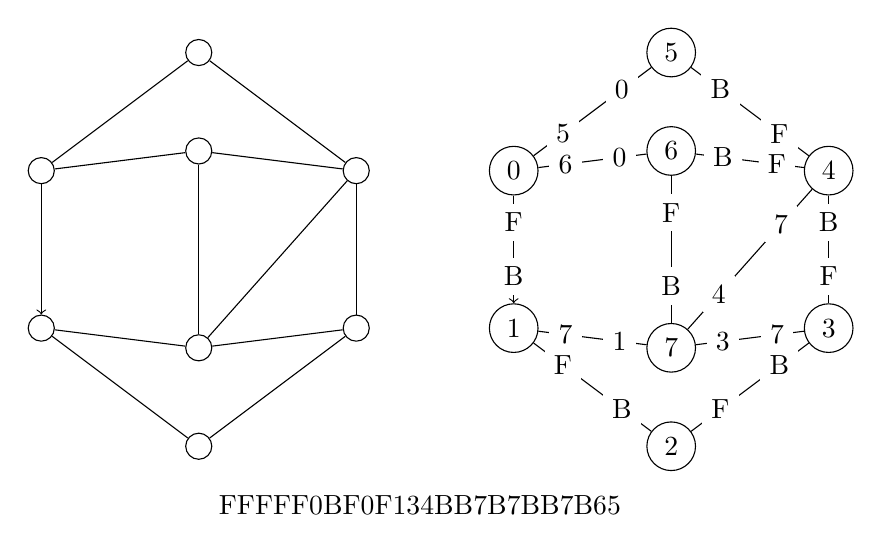
\begin{tikzpicture}[main/.style = {draw, circle, fill=white}]

		\node[main] (0) at (-2, 2) {};
		\node[main] (1) at (-2, 0) {};
		\node[main] (2) at (0, -1.5) {};
		\node[main] (3) at (2, 0) {};
		\node[main] (4) at (2, 2) {};
		\node[main] (5) at (0, 3.5) {};
		\node[main] (6) at (0, 2.25) {};
		\node[main] (7) at (0, -0.25) {};
		
		\draw[->] (0) -- (1);
		\draw (1) -- (2) ;
		\draw (2) -- (3) ;
		\draw (3) -- (4) ;
		\draw (4) -- (5) ;
		\draw (5) -- (0) ;
		\draw (4) -- (6) ;
		\draw (6) -- (0) ;
		\draw (6) -- (7) ;
		\draw (7) -- (1) ;
		\draw (7) -- (3) ;
		\draw (7) -- (4) ;
		
		
		
	
	
		\node[main] (0A) at (4, 2) {0};
		\node[main] (1A) at (4, 0) {1};
		\node[main] (2A) at (6, -1.5) {2};
		\node[main] (3A) at (8, 0) {3};
		\node[main] (4A) at (8, 2) {4};
		\node[main] (5A) at (6, 3.5) {5};
		\node[main] (6A) at (6, 2.25) {6};
		\node[main] (7A) at (6, -0.25) {7};
		
		\draw[->] (0A) -- (1A) node [near start, fill=white] {F} node [near end, fill=white] {B};
		\draw (1A) -- (2A) node [near start, fill=white] {F} node [near end, fill=white] {B};
		\draw (2A) -- (3A) node [near start, fill=white] {F} node [near end, fill=white] {B};
		\draw (3A) -- (4A) node [near start, fill=white] {F} node [near end, fill=white] {B};
		\draw (4A) -- (5A) node [near start, fill=white] {F} node [near end, fill=white] {B};
		\draw (5A) -- (0A) node [near start, fill=white] {0} node [near end, fill=white] {5};
		\draw (4A) -- (6A) node [near start, fill=white] {F} node [near end, fill=white] {B};
		\draw (6A) -- (0A) node [near start, fill=white] {0} node [near end, fill=white] {6};
		\draw (6A) -- (7A) node [near start, fill=white] {F} node [near end, fill=white] {B};
		\draw (7A) -- (1A) node [near start, fill=white] {1} node [near end, fill=white] {7};
		\draw (7A) -- (3A) node [near start, fill=white] {3} node [near end, fill=white] {7};
		\draw (7A) -- (4A) node [near start, fill=white] {4} node [near end, fill=white] {7};
		
		
		\node[] at (2.75, -2.25) {$\implies$ FFFFF0BF0F134BB7B7BB7B65};

\end{tikzpicture}
\caption{Example of a DFS traversal transcript for a graph. It is the lexicographically smallest transcript in this case.}
\end{figure}


We compute such string for all the edges of the outer face as starting edges, and we take the lexicographically smallest one as the canonical form. It is clear that
two plane graphs have the same canonical string if and only if they have isomorphic (in terms of the rotation system) embeddings. 

\todo{Maybe be more explicit with the explaination of the canonical form, and indeed prove that it is canonical}.

\section{Generation of Critical Cycle-Canvases}

Our algorithm for the generation of critical cycle-canvases is based on \ref{cyclechordtripodtheorem}. 
This theorem says that every critical cycle-canvas can either be decomposed into two smaller critical 
cycle-canvases through a chord in the outer face, it can be decomposed into a ``tripod'', a vertex $v$ 
with at least $3$ neighbors in $C$, and a smaller critical cycle-canvas contained in the only nonempty 
face incident with $v$. In these decompositions, it is possible that instead of a smaller critical canvas 
we get an empty canvas, which is technically not critical. \todo{check that all definitions of critical 
canvases are consistent with this}

This implies that we can generate all critical cycle-canvases from smaller cycle-canvases by gluing
cycle-canvases through outer face edges to get a canvas with a chord, or by adding a tripod to the
outside of a cycle-canvas. We then have to check whether the resulting canvas is indeed critical,
since the decomposition into two smaller critical cycle-canvases is a necessary but not sufficient condition
for criticality. We will see how to do this in Section 4. \todo{references for sections}.

\missingfigure{The three cases for generation of critical cycle-canvases}

\todo{figure for generation of critical cycle-canvases and references to figure}

If we are generating cycle-canvases with cycle length $\ell$, then a chord partitions
the cycle-canvas into two cycle-canvases of length $a$, $b$ with $a, b \geq 3$ and $a + b = \ell + 2$ (see figure (a)), so 
$a, b \leq \ell-1$ and therefore if we have generated all cycle-canvases with cycle length $< \ell$ we can generate
all cycle-canvases with cycle length $\ell$ with a chord. In the case of adding a tripod, though, if the vertex $v$ of
the tripod is adjacent to only three adjacent vertices in the outer face, then the smaller cycle-canvas has the same
cycle length as the larger cycle-canvas (see figure (c)).

In order to resolve this, what we do is first generate all the cycle-canvases obtained from cycle-canvases with smaller cycle size 
(as in figure (a) and (b)), enqueue the resulting critical canvases, and then process the canvases from the queue and add tripods 
to three consecutive vertices in all possible ways, enqueueing the new critical cycle-canvases that are found. Here is the description 
of the algorithm:

\todo{Fix lines with comments having semicolon in algorithms}

\begin{algorithm}[H]
\caption{Generation of Critical Cycle-Canvases.}
\SetAlgoLined
\SetKwComment{Comment}{/* }{ */}
\SetKwProg{Fn}{function}{}{end}
\Comment*[h]{Generate critical canvases of cycle size $\ell$, including empty one}

\Fn{generateCriticalCycleCanvases($\ell$)}{ 
	
	\For{$i = 3, \ldots, \ell-1$} {
		$S_i \gets \text{generateCriticalCycleCanvases}(i)$\;
	}
	$S \gets \{ \text{emptyCycle}(\ell) \}$\;
	
	\For{$a = 3, \ldots, \ell-1$} {
		$b \gets \ell-a+2$\;
		\For{$G_1 \in S_a$} {
			\For{$G_2 \in S_b$} {
				$T \gets \text{fuseChordSet}(G_1, G_2)$\; 
				\Comment*[r]{Set of cycle-canvases obtained by fusing $G_1$ and $G_2$ along outer cycle edges in all possible ways}
				\For{$G \in T$} {
					\If{$G \not\in S$ AND $\text{isCritical}(G)$} {	
						$S \gets S \cup \{G\}$\;
					}
				} 
			}
		}
	}
	\For{$k = 3, \ldots, \ell-1$} {
		\For{$G_1 \in S_k$} {
			$T \gets \text{addTripodSet}(G_1, \ell-k+3, 3)$\;
			\Comment*[r]{Set of cycle-canvases obtained by adding a tripod with $3$ neighbors in the outer face to get a cycle-canvas of length $\ell$ in all possible ways}
			\For{$G \in T$} {
				\If{$G \not\in S$ AND $\text{isCritical}(G)$} {	
					$S \gets S \cup \{G\}$\;
				}
			} 
		}
	}	
	$Q \gets \text{Queue}(S)$\; 
	\While{$Q \text{ is not empty}$} {
		$G_1 \gets \text{first}(Q)$\;
		$\text{dequeue}(Q)$\;
		$T \gets \text{addTripodSet}(G_1, 3, 3)$\;
		\For{$G \in T$} {
			\If{$G \not\in S$ AND $\text{isCritical}(G)$} {	
				$S \gets S \cup \{G\}$\;
				$\text{enqueue}(Q, G)$\;
			}
		} 
	}
	return $S$\;
}


\end{algorithm}

\todo{fix algorithm size}


Note that we only need to add tripods with $3$ adjacent neighbors since vertices with a larger number of neighbors in the
outer face can be obtained by first adding chords and then adding finally adding a tripod with $3$ neighbors. However, 
often we are interested in just generating chordless critical canvases. In that case, we do need to add tripods of all sizes.
The modified algorithm for chordless critical cycle-canvases is the following:

\begin{algorithm}[H]
\caption{Generation of Chordless Critical Cycle-Canvases.}
\SetAlgoLined
\SetKwComment{Comment}{/* }{ */}
\SetKwProg{Fn}{function}{}{end}
\Comment*[h]{Generate chordless critical canvases of cycle size $\ell$, including empty one}

\Fn{generateChordlessCriticalCycleCanvases($\ell$)}{ 
	
	\For{$i = 3, \ldots, \ell-1$} {
		$S_i \gets \text{generateChordlessCriticalCycleCanvases}(i)$\;
	}
	$S \gets \{ \text{emptyCycle}(\ell) \}$\;
	\For{$k = 3, \ldots, \ell-1$} {
		\For{$j = 3, \ldots, \ell-k+3$} {
			\For{$G_1 \in S_k$} {
				$T \gets \text{addTripodSet}(G_1, \ell-k+3, j)$\;
				\For{$G \in T$} {
					\If{$G \not\in S$ AND $\text{isCritical}(G)$} {	
						$S \gets S \cup \{G\}$\;
					}
				} 
			}
		}
	}	
	$Q \gets \text{Queue}(S)$\; 
	\While{$Q \text{ is not empty}$} {
		$G_1 \gets \text{first}(Q)$\;
		$\text{dequeue}(Q)$\;
		$T \gets \text{addTripodSet}(G_1, 3, 3)$\;
		\For{$G \in T$} {
			\If{$G \not\in S$ AND $\text{isCritical}(G)$} {	
				$S \gets S \cup \{G\}$\;
				$\text{enqueue}(Q, G)$\;
			}
		} 
	}
	return $S$\;
}


\end{algorithm}


\section{Generation of Critical Wedges}
\label{sec:generationwedges}

We are will be not only interested in generating critical cycle-canvases, but also critical path-canvases or wedges. 
There are infinitely many of those for path length greater than $1$, but as we will see in coming sections, 
we will be able to have a finite number of them if we impose additional conditions. 

Fortunately, we also have an analogue of theorem \ref{cyclechordtripodtheorem} for wedges:

\begin{theorem}[Wedge Chord or Tripod Theorem]
If $(G, P, L)$ is a $2$-connected critical wedge, then either

\begin{enumerate}
\item The outer walk $C$ has a chord in $G$, or
\item there exists a vertex $v \in V(G) \setminus V(P)$ with at least three neighbors on $P$ such that at most one of the faces of 
$G[\{v\} \cup V(P)]$ includes a vertex or edge of $G$. 
\end{enumerate}
\end{theorem}

\begin{proof}
Assume not. Then, we will show that every $L$-coloring of $P$ extends to an $L$-coloring of $G$, contradiction. Let $\phi$ be any $L$-coloring of $P$, 
$G' = G \setminus P$ and $L'(v) = L(v) \setminus \{\phi(u) : u \in V(P) \text{ neighbor of } v \}$ for each $v \in V(G')$. 
Note that $|L'(v)| \geq 5$ for every interior vertex of $G'$. Let $C'$ be the outer walk of $G'$ and let $v_1$, $v_2$ be the two vertices of 
$G'$ that were adjacent to the two endpoints of $P$ in $G$. Note that $|L'(v)| \geq 3$ for all $v \in C' \setminus \{v_1, v_2\}$ since 
$G$ was $2$-connected and had no chords, and $|L(v_1)|, |L(v_2)| \geq 2$. Hence, $G'$ is $L'$-colorable by \ref{twolistsofsizetwo}.
\end{proof}

(This version of the theorem is slightly different than the one proved by Postle in \cite{postlethesis}).

Based on this theorem, we can design an algorithm to generate critical wedges similar to the one used to generate critical canvases.  
The main additional consideration we need to take into account is that now we need to generate non-$2$-connected critical wedges by 
gluing smaller critical wedges along the cutvertices. Observe that the cutvertices must necessarily be part of $P$.

\todo{Fix critical wedges algorithm}

\begin{algorithm}[H]
\caption{Generation of Critical Wedges.}
\SetAlgoLined
\SetKwComment{Comment}{/* }{ */}
\SetKwProg{Fn}{function}{}{end}
\Comment*[h]{Generate critical wedges of path size $\ell$, including the path}

\Fn{generateCriticalWedges($\ell$)}{ 
	
	\For{$i = 3, \ldots, \ell-1$} {
		$S_i \gets \text{generateCriticalCycleCanvases}(i)$\;
	}
	$S \gets \{ \text{emptyPath}(\ell) \}$\;
	
	\For{$a = 3, \ldots, \ell-1$} {
		$b \gets \ell-a+2$\;
		\For{$G_1 \in S_a$} {
			\For{$G_2 \in S_b$} {
				$T \gets \text{fuseChordSet}(G_1, G_2)$\; 
				\Comment*[r]{Set of cycle-canvases obtained by fusing $G_1$ and $G_2$ along outer cycle edges in all possible ways}
				\For{$G \in T$} {
					\If{$G \not\in S$ AND $\text{isCritical}(G)$} {	
						$S \gets S \cup \{G\}$\;
					}
				} 
			}
		}
	}
	\For{$k = 3, \ldots, \ell-1$} {
		\For{$G_1 \in S_k$} {
			$T \gets \text{addTripodSet}(G_1, \ell-k+3, 3)$\;
			\Comment*[r]{Set of cycle-canvases obtained by adding a tripod with $3$ neighbors in the outer face to get a cycle-canvas of length $\ell$ in all possible ways}
			\For{$G \in T$} {
				\If{$G \not\in S$ AND $\text{isCritical}(G)$} {	
					$S \gets S \cup \{G\}$\;
				}
			} 
		}
	}	
	$Q \gets \text{Queue}(S)$\; 
	\While{$Q \text{ is not empty}$} {
		$G_1 \gets \text{first}(Q)$\;
		$\text{dequeue}(Q)$\;
		$T \gets \text{addTripodSet}(G_1, 3, 3)$\;
		\For{$G \in T$} {
			\If{$G \not\in S$ AND $\text{isCritical}(G)$} {	
				$S \gets S \cup \{G\}$\;
				$\text{enqueue}(Q, G)$\;
			}
		} 
	}
	return $S$\;
}


\end{algorithm}

